
% this file is called up by thesis.tex
% content in this file will be fed into the main document

% ----------------------- introduction file header -----------------------
%\chapter{Search for the FCNC decay \pmb{$t\rightarrow c + Z$}}
\chapter{Search for FCNC top quark decay $t\rightarrow cZ$}
\label{chapter:analysis}
This chapter presents a search for flavour-changing neutral current top-quark decay $t\rightarrow cZ$.\\ 
The study uses a data sample from proton--proton collisions at 
$\sqrt{s}$ = \SI{13}{\TeV} recorded in full Run2 (from 2015 to 2018) by the ATLAS experiment, and targets final states with three
leptons (either electrons or muons).\\
I took in charge of most of the analysis, from the event selection up to the extraction of the final results.\\

% ----------------------- paths to graphics ------------------------

% the code below specifies where the figures are stored
\graphicspath{Chapters/CH5/figures}

% ----------------------------------------------------------------------
% ----------------------- introduction content -------------------------
% ----------------------------------------------------------------------

\section{Physics motivation}
The heaviest particle in the Standard Model (SM), the top quark, decays almost exclusively to a \PW-boson and a bottom quark~\cite{pdg2}. In proton--proton ($pp$) collisions, top quarks are produced dominantly in pairs, via the strong interaction, but also singly, via the electroweak interaction. \\%involving a $Wtb$ vertex. %Therefore single-top quark production provides a powerful probe of the electroweak couplings of the top quark. 
Within the SM, "flavour-changing neutral-current" (FCNC) processes are forbidden at tree level due to the Glashow-Iliopoulos-Maiani mechanism \cite{gim} (see Section~\ref{sec:gim}) and the approximate diagonality of the Cabibbo-Kobayashi-Maskawa matrix~\cite{pdg2} causes the suppression of such processes at higher orders (see Section~\ref{sec:ckm}).\\
Nonetheless, there are several scenarios beyond the Standard Model (BSM) that can significantly enhance the FCNC processes in the top quark sector, opening a door for its detection at the Large Hadron Collider (LHC)~\cite{aguilar,barger,h2dm_limit,mssm_limit,RPV_limit, extra_limit} and some of them have been already discussed in Section~\ref{sec:bsm}. \\
The analysis presented in the following searches for FCNC \tZc coupling. A comparison between SM and BSM predictions for the branching ratios of top quark decays to an up or a charm quark and a \PZ boson is shown in Table \ref{tab:intro-fcnc-br-th}.\\

\begin{table}[h]
	\begin{adjustbox}{max width=1.\textwidth,center}
		\begin{tabular}{ccccccccc}
			\hline 
			Model:&  			                         SM&  				   QS&  			   2HDM&  				FC 2HDM				& MSSM 			&  RPV SUSY			&  			RS				& EMF \\ 
			\hline 
			$\mathcal{B}(t\rightarrow qZ)$ & $10^{-14}$     & $10^{-4}$ &  $10^{-6}$          & $10^{-10}$  & $10^{-7}$      &$10^{-6}$            & $10^{-5}$           & $10^{-6}$  \\ 
			\hline 
		\end{tabular} 
	\end{adjustbox}
	\caption{Maximum allowed FCNC $t\rightarrow qZ$, ($q$ = $u$, $c$) branching ratios predicted by several models\cite{tcZ_sm,qs_limit,h2dm_limit,mssm_limit,RPV_limit,extra_limit,rs_limit,report_limit}.}
	\label{tab:intro-fcnc-br-th}
\end{table} 

\begin{figure}[htb]
	\centering
	\subfigure[Single top production via FCNC ($s$-channel)]{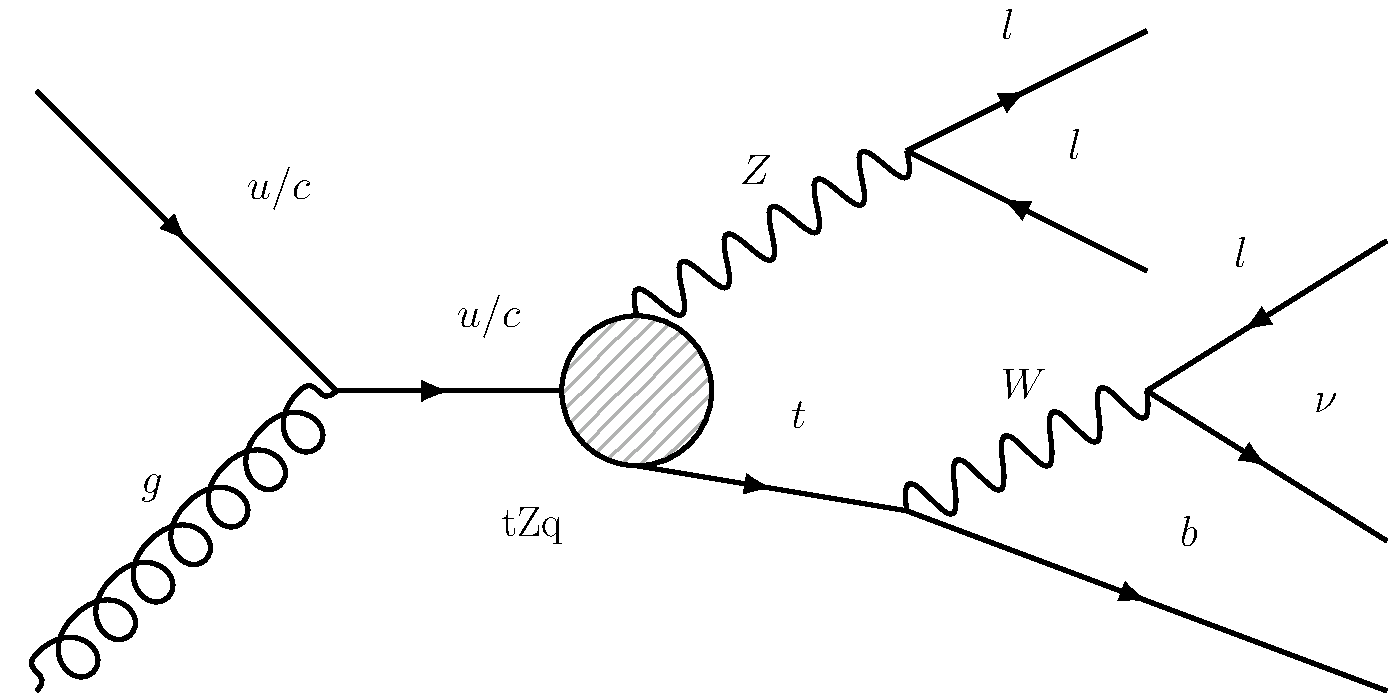
\includegraphics[width=0.50\textwidth]{Chapters/CH5/figures/Production_1.pdf}\label{subfig:signal1}}\qquad
	\subfigure[Single top production via FCNC ($t$-channel)]{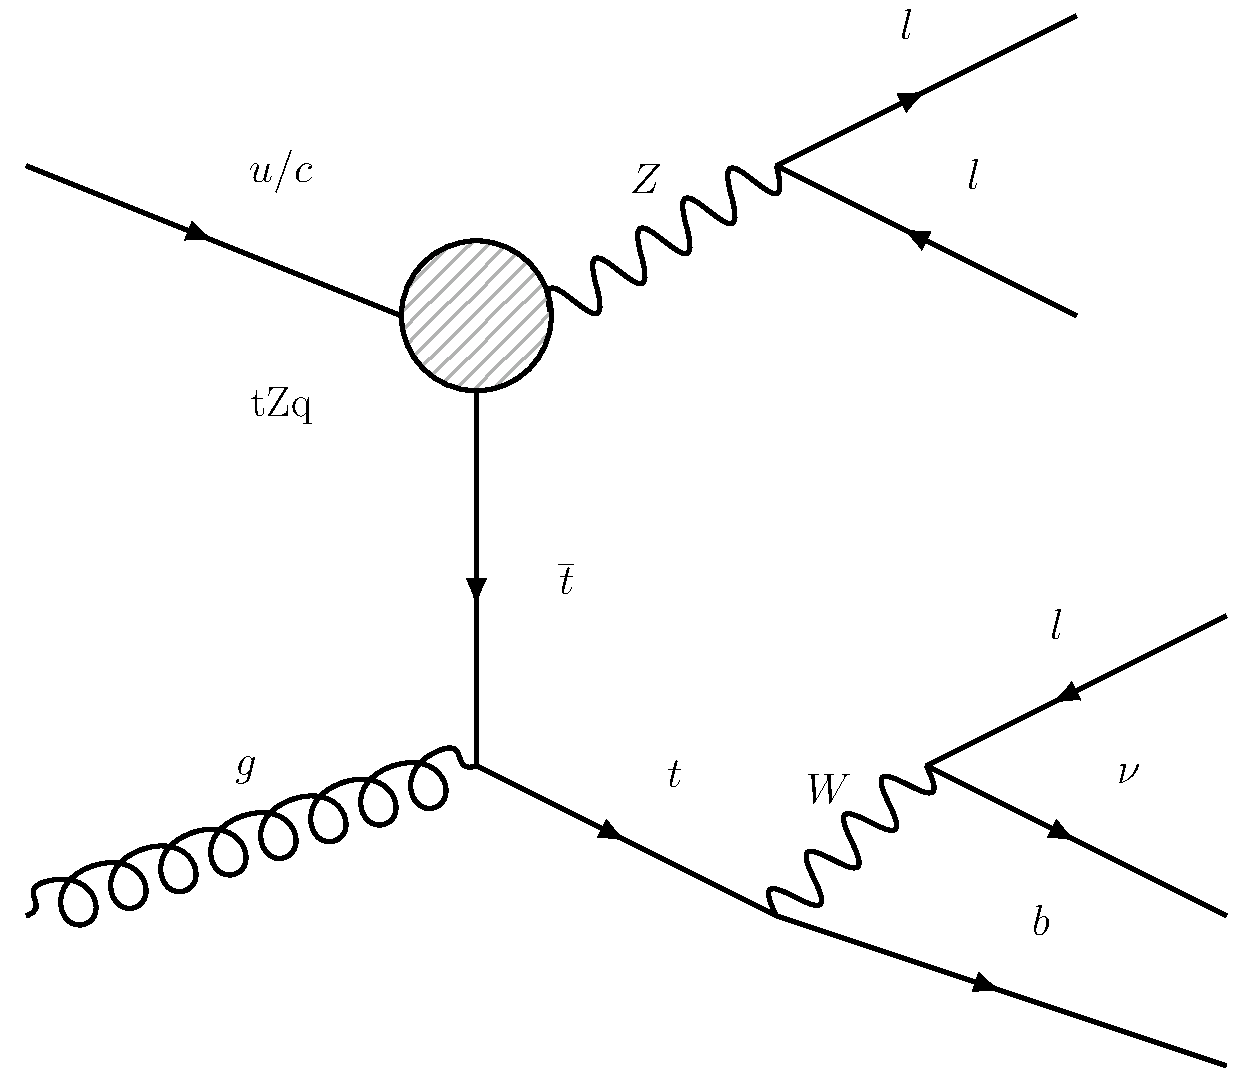
\includegraphics[width=0.40\textwidth]{Chapters/CH5/figures/Production_2.pdf} \label{subfig:signal2} }
	\subfigure[ \ttbar production with \tZc decay]{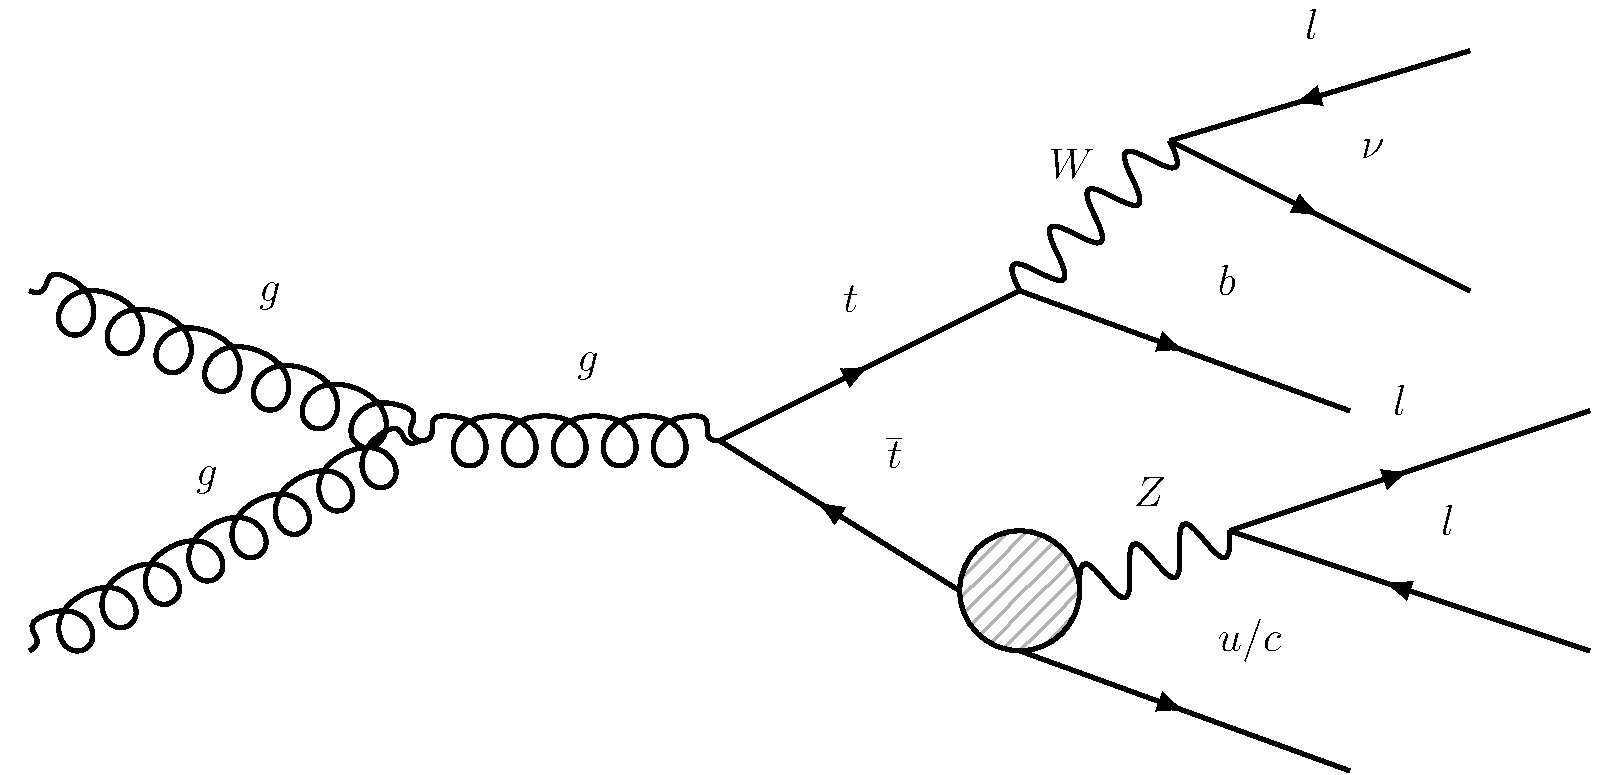
\includegraphics[width=0.54\textwidth]{Chapters/CH5/figures/TtbarProduction.pdf} \label{subfig:signal3}}
	\caption{Examples of lowest order Feynman diagrams for single top production via FCNC in \subref{subfig:signal1} the $s$-channel and \subref{subfig:signal2} the $t$-channel. Example of the lowest order Feynman diagrams for \subref{subfig:signal3} \ttbar production, with one top-quark decaying through the SM and the other via \tZc coupling. The vertex labelled as \tZq corresponds to the coupling responsible for the FCNC interaction.}
	\label{fig:signal}
\end{figure} 

\noindent In a model independent way, the anomalous couplings can be described by the so called effective field theory (EFT).
This theory considers an extension of the SM Lagrangian $\mathcal{L}_{SM}$ by operators in higher-dimensions of the mass suppressed by the scale of new physics $\Lambda$ as shown in \Cref{eq:lagrangian}.
Dimension-5 operators are not considered in this analysis due to the introduction of lepton-flavour violating processes. 
Therefore, the anomalous couplings can be approximated with dimension-6 operators $O_{i}^{(6)}$ whose strength  is given by the Wilson coefficients $C_{i}^{(6)}$.\\

\begin{equation}
\mathcal{L} = \mathcal{L}_{SM} + \frac{1}{\Lambda^2}\sum_{i} C_{i}^{(6)} O_{i}^{(6)}  
\label{eq:lagrangian}
\end{equation}

\noindent Experimental limit on the branching ratio of FCNC $t\rightarrow cZ$ decays was previously established by experiments at the Large Electron-Positron Collider (LEP)~\cite{ALEPH,DELPHI,OPAL,L3}, the Hadron-Electron Ring Accelerator (HERA)~\cite{ZEUS}, the Tevatron\ \cite{CDF,DZero} and the Large Hadron Collider (LHC)~\cite{TOPQ-2017-06,Chatrchyan:2013nwa,CMS-TOP-12-039}. The ATLAS and the CMS collaborations obtained limits at the \SI{95}{\percent} confidence level (CL) for this process using data collected at $\sqrt{s}$ = \SI{13}{\TeV} and $\sqrt{s}$ = \SI{8}{\TeV}, focusing on FCNC top-quark decays~\cite{TOPQ-2017-06,Chatrchyan:2013nwa}, or both production and decay modes combined~\cite{CMS-TOP-12-039}. 
A summary of the ATLAS and CMS results on the limits on FCNC couplings is shown in \Cref{fig:intro:limits}. The actual observed limits on the FCNC \tZc coupling from ATLAS is $\mathrm{BR(t\to cZ) < \SI{2.4e-4}{}}$~\cite{TOPQ-2017-06}.\\
Recent studies were done on the interference effects on the \textit{tZ1} and $t\gamma q$ anomalous couplings, concluding that these effects are smaller than the variations of the systematics uncertainties considered~\cite{Interference}. Therefore, both decay and production modes are taken into account in this analysis to improve the results on the limit for \tZc anomalous coupling.

\begin{figure}[htb]
	\centering
	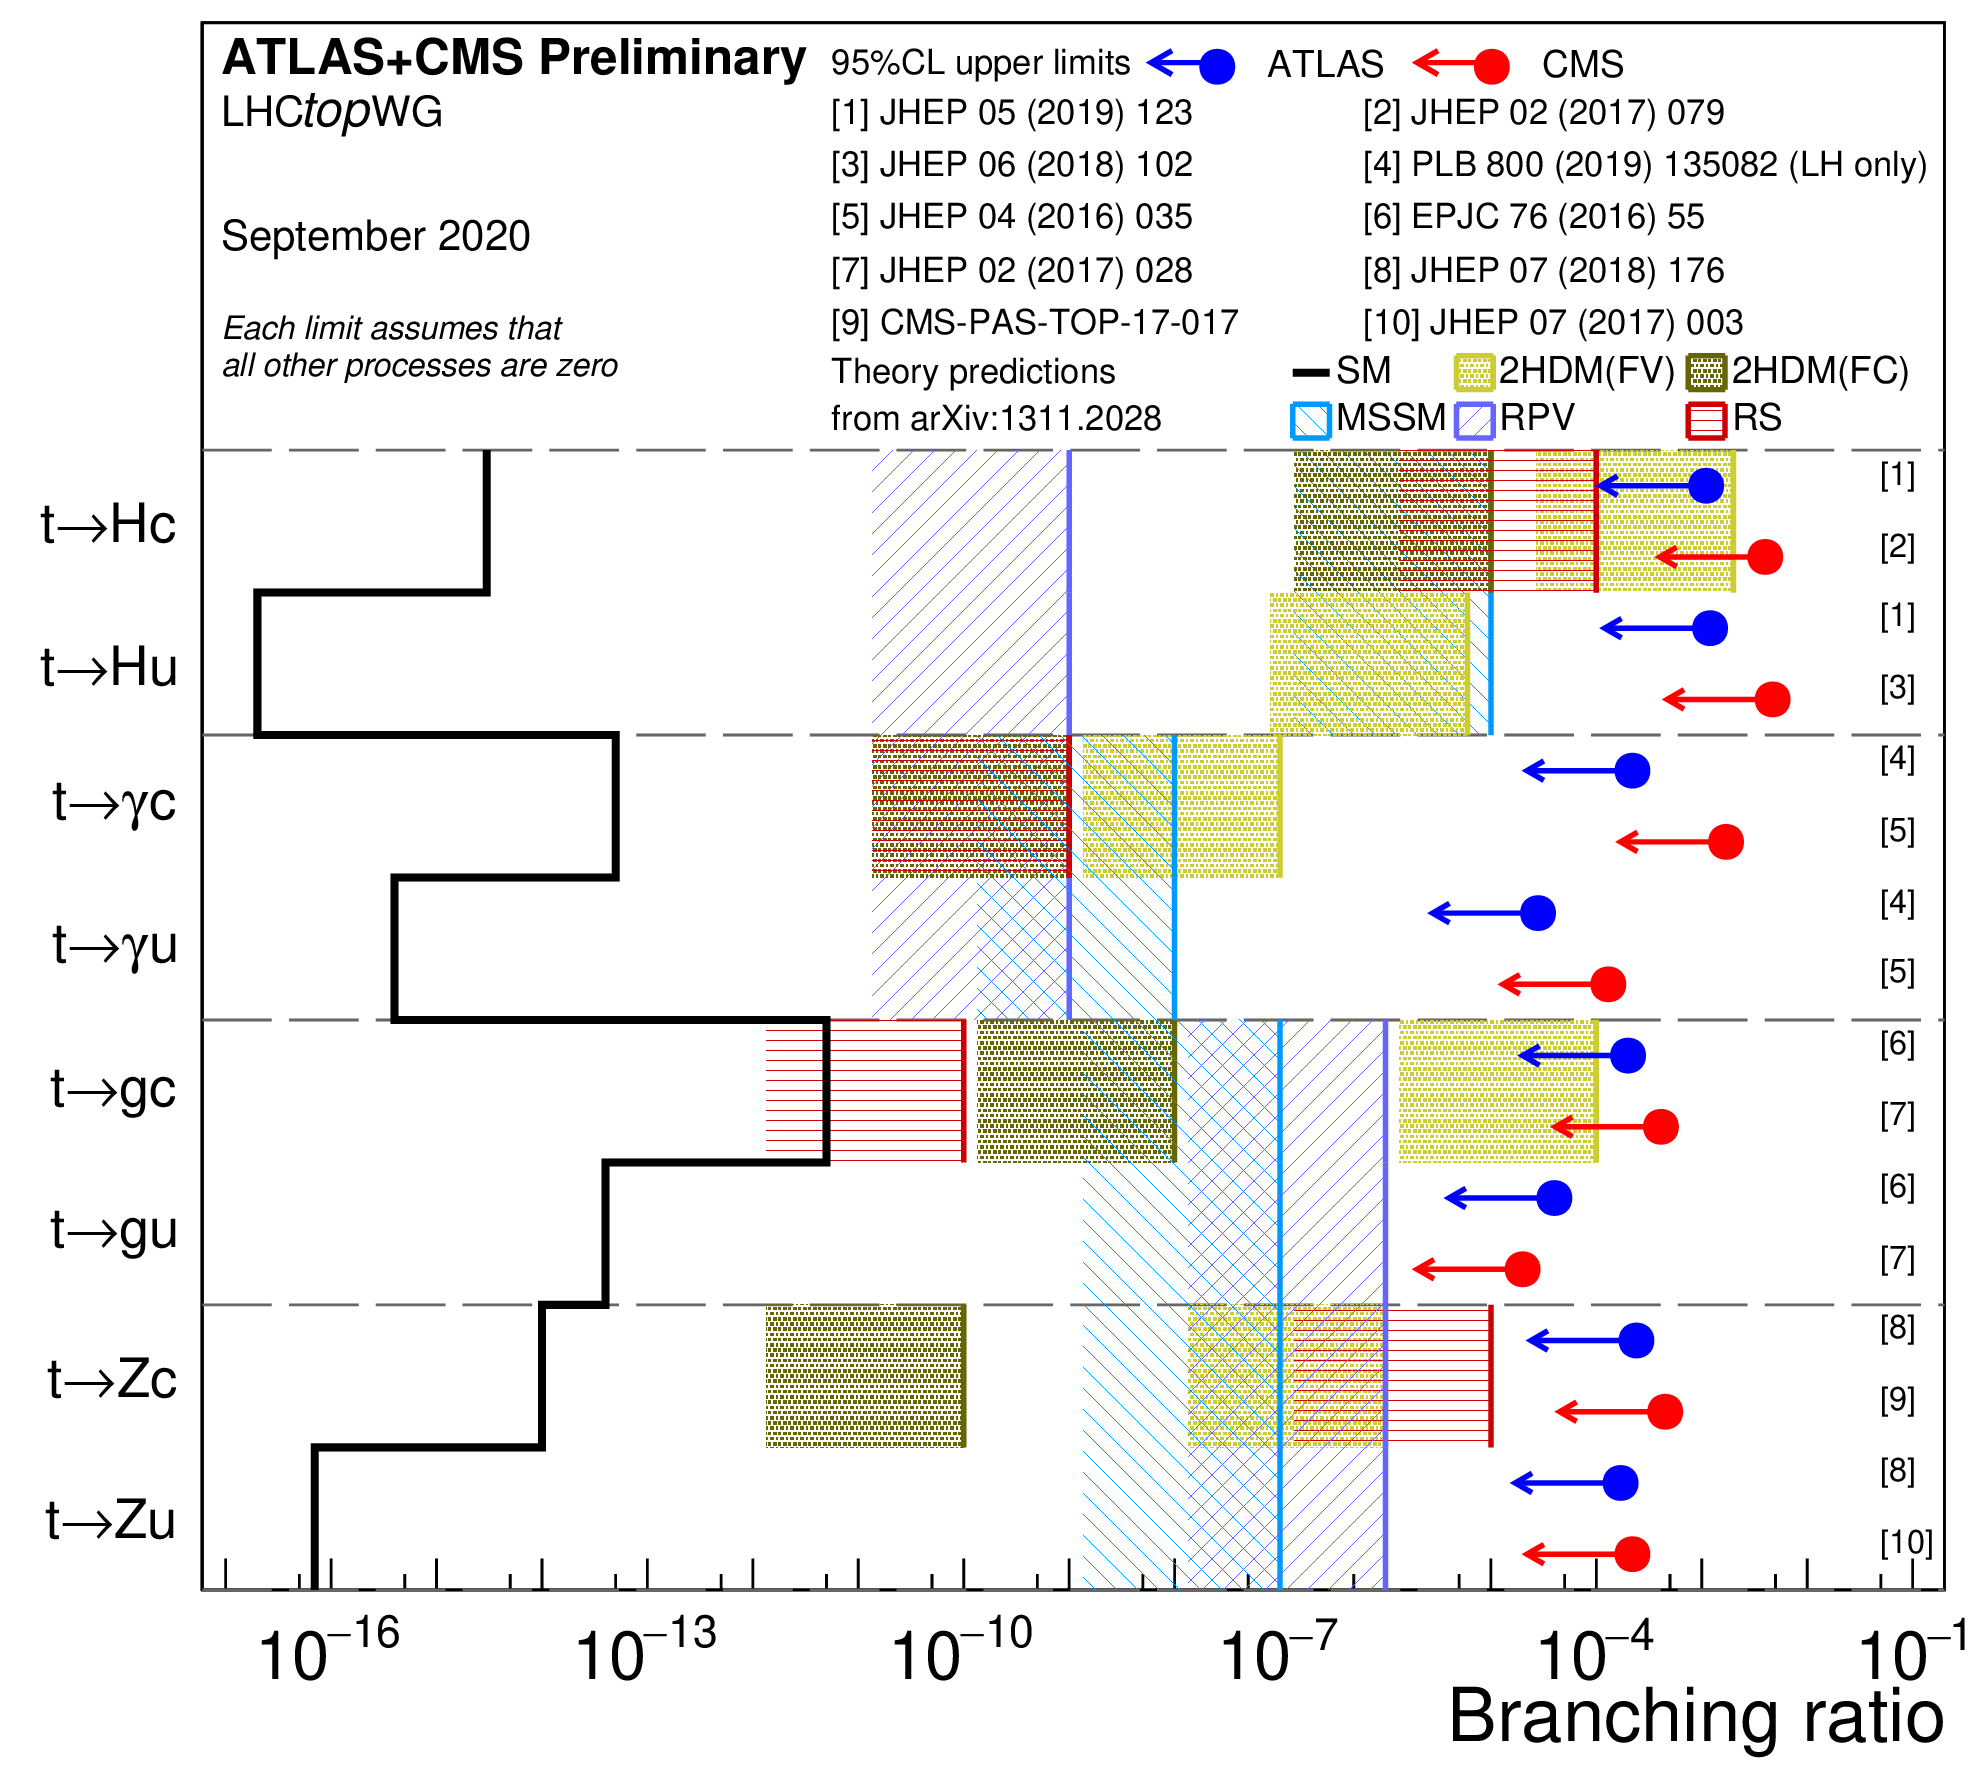
\includegraphics[scale=0.15]{Chapters/CH5/figures/fcnc_summarybsm}
	\caption{Summary of the current 95\% confidence level observed limits on the branching ratios of the top quark decays via flavour changing neutral currents to a quark and a neutral boson $t\rightarrow Xq$ ($X = g, Z, \gamma,$ or $H$; $q = u$ or $c$) by the ATLAS and CMS Collaborations compared to several new physics models. The ATLAS limits on $t \rightarrow q$ are valid for the case of a purely left-handed coupling. Status of figure: September 2019 (Top2019)}
	\label{fig:intro:limits}
\end{figure}

\clearpage
\section{Analysis strategy}
In the following, the analysis strategy is described.

\paragraph{Analysis overview}
The analysis presented in the following searches for flavour-changing
neutral current (FCNC) coupling between the top-quark and the \PZ
boson in proton--proton collisions at $\sqrt{s} = \SI{13}{\TeV}$ with
the ATLAS detector. \\
The search is carried out in both single-top quark production and
top-quark pair-production events.\\
The search for FCNC $t\rightarrow cZ$ processes can be performed by analysing the top quark decays in \ttbar events as well as the production of single-top quarks (see Figure \ref{fig:signal}). In the former channel, one of the top quarks decays through FCNC and the other through the SM mode ($t\to Wb$). The latter channel is characterised by a final state composed of a single top quark and a \PZ boson. The main difference between the final states of decay and production modes is the presence of one additional jet. \\
The analysis presented in the following targets both production and decay mode. This search is done using $pp$ collision data collected by the ATLAS detector at a centre-of-mass energy of \SI{13}{\TeV} and corresponding to an integrated luminosity of \lumi.\\
The analysis targets both events with the production of a \PZ boson and a single-top quark decaying to a \PW boson and a \Pqb-quark and events with the production of top quark pairs, where one top quark decays to a \PZ boson and a charm quark and the other top quark decays to a \PW boson and a \Pqb-quark. For both modes, the \PZ boson decays into two charged leptons (electrons or muons including those coming from leptonic $\tau$-lepton decays) and the \PW boson from the top quark decays leptonically too. \\
In addition, to increase the sensitivity to FCNC \tZc couplings, 
a charm tagging technique is exploited for
the semi-leptonic decays of \Pqc-hadrons produced by the FCNC top
decay. 

\paragraph{Dataset}
Data from proton--proton collisions at 
$\sqrt{s}$ = \SI{13}{\TeV} recorded in full Run2 (from 2015 to 2018) by the ATLAS experiment is used, for a total integrated luminosity of \lumi.\\
The description of the data and Monte Carlo samples used in the following can
be found in \Cref{sec:samples}.

\paragraph{Signal regions}
Three Signal Regions (SRs) are defined for the \tZc coupling extraction, targeting:
\begin{itemize}
	\item FCNC \tZc in \ttbar decays (called SR1\tZc), 
	\item FCNC \tZc in single-top production (called SR2\tZc), 
	\item FCNC \tZc in \ttbar decays (called SR3\tZc) using either:
	\begin{itemize}
		\item the SMT technique or
		\item the \Pqc-tagger \DLrc
	\end{itemize}
\end{itemize}
The SRs are orthogonal between each other. 
%The orthogonality is assured by selecting events with different jet multiplicities and by selecting or vetoing the presence of a jet associated to a soft muon.\\
The main focus of this thesis is the definition of SR3\tZc investigating the best c-tagging technique for this analysis.\\
The event selection using the SMT technique is reported in \Cref{sec:selection}.\\
The event selection using $\mathrm{DL1r_{c}}$ tagger is reported in \Cref{sec:other_selection}, together with the comparison with SMT.\\
The description of the other SRs selections, used to extract expected limits, is reported in \Cref{sec:selection_all}.\\

\paragraph{Background estimation}
The main background sources are:
\begin{itemize}
	\item for SR1\tZc, \ttZ and Diboson (VV)+HF;
	\item for SR2\tZc, \VVHF and Standard Model \tZq ;
	\item for SR3\tZc, \ttZ and Diboson (VV)+HF.
\end{itemize}

\noindent All backgrounds are estimated using Monte Carlo samples. They are
normalised to the theoretical cross-sections. 
%The normalisation of the \ttbar background is left free floating in the fits.
Various control regions (CRs) are constructed to control the
background normalisations. A total of four CRs is used. 
The description of the background sources and the CR selections is
reported in \Cref{sec:background}.

\paragraph{Separation of signal and backgrounds}
A multivariate analysis is used to improve the discrimination of
signal to background events providing SRs with increased \ssb. \\
Gradient Boosted Decision Trees (GBDTs) are trained separately for each SR. \\
The description of the multivariate analysis can be found in
\Cref{sec:separation}. 

\paragraph{Fit and limit extraction}
To extract limits on the FCNC \tZc coupling, the output of the
GBDT in the SRs are simultaneously fit, together with other 
distributions in the CRs. 

\noindent The description of the fit and of the extraction of the limits can be
found in \Cref{chapter:Statistical_analysis}.

\paragraph{Blinding strategy}
A blinding strategy is set to reduce any possible bias in the measurement. 
The prescriptions of the Top Working Group are followed~\cite{top:blind}.\\
To make sure that the background sources are correctly described,
data is only looked at in regions where the signal contribution is expected to be small, while 
\textit{pseudo-data}, called \textit{Asimov data} are used in Signal Regions (see \Cref{sec:stat:tzc:splusb:crsr}). 

\section{Data and Monte Carlo samples}
\label{sec:samples}
This section describes the samples used in this analysis.
The detailed lists of data and Monte Carlo (MC) samples can be found
in \App{\ref{appendix:app_mc}}, 
while a description is presented below.\\
The starting point for the analysis are the ROOT~\cite{Antcheva:2009zz} ntuples, produced using the common ATLAS software version
\anabasevers, starting from \texttt{TOPQ1} derivations~\cite{top:deriv}.\\
The derivations contain a filter that requires at least one lepton
(a loose electron or a good combined muon) with a \pT above \SI{20}{\GeV} and $\abseta \leq 2.5$. 

%-------------------------------------------------------------------------------
\subsection{Data sample}%
\label{sec:samples:data}
%-------------------------------------------------------------------------------

The analysis described in this paper uses data collected from 2015 to 2018 by the ATLAS detector at a centre-of-mass energy of \SI{13}{\TeV}.
The complete sample includes all \SI{25}{\nano\second} data periods from 2015, as well as the whole 2016--2018 datasets.
The total integrated luminosity is of \lumi.
The selected data periods were collected during stable beam LHC operations and with the ATLAS detector fully functioning.\\
The partial integrated luminosities and the Good Run Lists\footnote{The Good Runs List (GRL) is a file that selects good luminosity blocks from within the data runs (spanning 1-2 minutes of data-taking). } (GRL) used are reported in \cref{tab:samples:lumi}. 

\begin{table}[htbp]
	\centering
	\small
	\begin{tabular}{cSl}
		\toprule
		Year & {Int.\ lumi.\ (\si{\ifb})} & GRL \\
		\midrule
		2015 & 3.2    & data15\_13TeV/20170619/physics\_25ns\_21.0.19.xml \\
		2016 & 33.0  & data16\_13TeV/20170605/physics\_25ns\_21.0.19.xml \\
		2017 & 44.3  & data17\_13TeV/20180619/physics\_25ns\_Triggerno17e33prim.xml \\
		2018 & 58.5  & data18\_13TeV/20181111/physics\_25ns\_Triggerno17e33prim.xml \\
		\bottomrule
	\end{tabular}
	\caption{Integrated luminosity per year.}%
	\label{tab:samples:lumi}
\end{table}

\noindent Events are considered only if they are accepted by at least one of the single-muon or single-electron triggers
described in Refs.~\cite{TRIG-2016-01,ATL-DAQ-PUB-2016-001,ATL-DAQ-PUB-2017-001,ATL-DAQ-PUB-2018-002} and listed in Table~\ref{tab:samples:trig}. \\
The ATLAS trigger system is composed by two levels: the first level (\texttt{L1}) is a hardware trigger implemented
in custom-built electronics, while the second level, referred to as high level trigger (\texttt{HLT}), is software based.

\begin{table}[htbp]
	\centering
	\footnotesize
	\begin{tabular}{cll}
		\toprule
		Year & \multicolumn{1}{l}{Single $e$} & \multicolumn{1}{l}{Single \Pgm} \\
		\midrule
		2015 & \texttt{HLT\_e24\_lhmedium\_L1EM20VH} & \texttt{HLT\_mu20\_iloose\_L1MU15} \\
		& \texttt{HLT\_e60\_lhmedium} & \texttt{HLT\_mu50} \\
		& \texttt{HLT\_e120\_lhloose} & \\
		\midrule
		2016--2018 & \texttt{HLT\_e26\_lhtight\_nod0\_ivarloose} & \texttt{HLT\_mu26\_ivarmedium} \\
		& \texttt{HLT\_e60\_lhmedium\_nod0} & \texttt{HLT\_mu50} \\
		& \texttt{HLT\_e140\_lhloose\_nod0} & \\
		\bottomrule
	\end{tabular}
	\caption{Trigger selections.}%
	\label{tab:samples:trig}
\end{table}

\noindent The electron triggers select a calorimeter cluster matched to a track.
Electrons must then satisfy identification criteria based on a multivariate technique using a likelihood (LH) discriminant.\\
In 2015, electrons had to satisfy a medium identification and have $\ET > \SI{24}{\GeV}$.\\
In 2016--2018, electrons had to satisfy a tight identification
together with an isolation criteria and have $\ET > \SI{26}{\GeV}$.
During the four years, to avoid efficiency losses due to identification and isolation at high \pT, 
two other triggers were also available,
selecting medium electrons with $\ET > \SI{60}{\GeV}$
and selecting loose electrons with $\ET > \SI{120}{\GeV}$ (\SI{140}{\GeV} in 2016--2018).\\
Muons are triggered on by matching tracks reconstructed in the muon spectrometer and in the inner detector.
In 2015, muons had to satisfy a loose isolation requirement and have $\pT >\SI{20}{\GeV}$. In 2016--2018, the isolation criterion was tightened and the threshold increased to $\pT >\SI{26}{\GeV}$.
During the four years, to avoid efficiency losses due to isolation at high \pT,
another muon trigger without any isolation requirement was available,
selecting muons with $\pT > \SI{50}{\GeV}$. 

%-------------------------------------------------------------------------------
\subsection{Monte Carlo simulated samples}%
\label{sec:samples:mc}
%-------------------------------------------------------------------------------

ATLAS Monte Carlo samples for analyses on the 2015--2018 dataset are split into three subsets: mc16a reflects the pile-up conditions of the years 2015 and 2016, mc16d reflects the pile-up conditions of 2017 data and mc16e reflects the pile-up conditions of 2018 data. Therefore, mc16a samples need to be scaled to 2015+2016 integrated luminosity, mc16d samples need to be scaled to 2017 integrated luminosity and mc16e samples need to be scaled to the 2018 integrated luminosity.\\
The generated MC samples containing top-quarks are produced with the top-quark mass, \mtop,
parameter set to \SI{172.5}{\GeV} and a branching fraction of the top-quark decay to a \PW boson and a \Pqb quark of 1. 
In all samples, decays into \Pgt leptons are included and if the \Pgt decays leptonically such events are taken into account in the analysis.\\
In the following, samples used in the analysis are explained in detail, both for the signal and for the background sources.

%-------------------------------------------------------------------------------
\subsubsection{Signal samples}
\label{sec:samples:mc:sig}
%-------------------------------------------------------------------------------

The Monte Carlo simulation samples for the signal were generated at next-to-leading order (NLO) with \aMCatNLO~\cite{Alwall:2014hca} interfaced to \PythiaEight~\cite{Sjostrand:2007gs} with the \textsc{A14} tune~\cite{Skands:2010ak} and the \textsc{NNPDF2.3LO} PDF set. Only decays of the \PW and \PZ bosons involving charged leptons were generated at matrix element level (\mbox{$Z\to e^+e^-,~\mu^+\mu^-,~\tau^+\tau^-$} and \mbox{$W \to e\nu, \mu\nu, \tau\nu$)}. For the matrix element, the PDF set \textsc{NNPDF3.0NLO} is used. The Universal FeynRules Output (UFO) model~\cite{Alloul:2013bka} is used for the computation at NLO in QCD. The top quark FCNC decay is done by TopFCNC model~\cite{Degrande:2014tta,Durieux:2014xla}.
The TopFCNC UFO model includes the effects of new physics at an energy scale $\Lambda$ by adding effective terms to the SM lagrangian:
\begin{equation}
\mathcal{L} = \mathcal{L}_{SM} + \mathcal{L}^{eff} = \mathcal{L}_4 + \frac{1}{\Lambda^2} \mathcal{L}_6+ ...
\end{equation}

\noindent where $\mathcal{L}_4$ = $\mathcal{L}_{SM}$ and $\mathcal{L}_6$ contains operators with dimension-six. The rest of the terms contain operators of dimension higher than 6 and will be suppressed due to the associated factors 1/$\Lambda^4$, ... $\mathcal{L}_6$ can be written as a linear combination of dimension-six operators $O_j$: 

\begin{equation}
\mathcal{L}_6 = \sum_j C_j O_j
\end{equation}

\noindent with $C_j$ being complex constants and $O_j$ being SM gauge invariant dimension-six operators that contain the fermion doublets and singlets, the gauge field tensors, the Higgs doublet and the covariant derivatives.\\
Taking into account that both production and decay modes are considered in this analysis, separated samples for each mode and for the \tZc (using $IC_{ctB}$ and $IC_{ctW}$) anomalous coupling were generated. In order to allow the study of the chirality of these couplings, samples with left-handed or right-handed couplings were obtained as well but the latter are not considered in this thesis.\\ Finally, an additional sample for \ttbar production was generated including a soft muon filter targeting the charm-tagged signal region. \\
Therefore, three different signal samples are considered:
\begin{itemize}
%	\item $tZ$ production for $tZu$ left-handed coupling; 
	\item $tZ$ production for \tZc left-handed coupling; 
%	\item \ttbar production for $tZu$ left-handed coupling; 
	\item \ttbar production for \tZc left-handed coupling; 
%	\item $tZ$ production for $tZu$ right-handed coupling; 
%	\item \ttbar production for $tZu$ right-handed coupling; 
	\item \ttbar production with soft muon tagging for \tZc left-handed coupling. 
\end{itemize}

\noindent For the signal samples with \ttbar production, it is considered that one of the top-quarks decays through FCNC to $cZ$ and the other, according to the SM, to $Wb$.\\ 
For the $tZ$ production, a top-quark and a \PZ boson is generated, where the top-quark decays according to the SM, since the $tZq$ anomalous coupling is assumed in the primary vertex. \\
The number of signal events is normalised to a branching ratio of  \mbox{BR($t\rightarrow cZ$) = $2.4\times10^{-4}$}, constraining \mbox{BR($t\rightarrow bW$) = 1 - BR($t\rightarrow cZ$).}\\
The considered value of the $t\to cZ$ branching ratio is the observed limit obtained from
the previous analysis at a center-of-mass energy of \SI{13}{\TeV} with \SI{36}{\ifb}~\cite{TOPQ-2017-06}. \\
The FCNC \ttbar decay signal
is normalised using the \ttbar cross-section prediction at next-to-next-to-leading order (NNLO)
in QCD including the re-summation of next-to-next-to-leading logarithmic (NNLL) soft-gluon terms calculated using
\textsc{Top++2.0}~\cite{Beneke:2011mq,Cacciari:2011hy,Baernreuther:2012ws,Czakon:2012zr,Czakon:2012pz,Czakon:2013goa,Czakon:2011xx}.
For proton--proton collisions at a centre-of-mass energy of \rts~=~\SI{13}{\TeV}, this cross section corresponds to
$\sigma(\ttbar)_{\textrm{NNLO+NNLL}} = \mathrm{832\pm51~pb}$ using a top-quark mass of $\mtop~ =~\SI{172.5}{GeV}$.\\
The uncertainties on the cross-section due to PDF and $\alpha_{\textrm{s}}$ are calculated using the PDF4LHC prescription~\cite{Botje:2011sn}
with the MSTW2008 68\% CL NNLO~\cite{Martin:2009iq,Martin:2009bu}, CT10 NNLO~\cite{Lai:2010vv,Gao:2013xoa} and \textsc{NNPDF2.3} 5f FFN~\cite{Ball:2012cx} PDF sets,
and are added in quadrature to the scale uncertainty.
The FCNC single-top quark production signal normalisation cross-section is calculated at 
NLO using the TopFCNC model as implemented in the \aMCatNLO.  \\

\subsubsection{Background samples}
\label{sec:samples:mc:bkg}
%-------------------------------------------------------------------------------

Simulated samples are included in the analysis in order to account for all the SM predicted background sources. 

\paragraph{$t\bar{t}$ production} 
The production of \ttbar\ events is modelled using the
\powhegbox~\cite{Frixione:2007nw,Nason:2004rx,Frixione:2007vw,Alioli:2010xd}~v2
generator at NLO with the \textsc{NNPDF3.0NLO}~\cite{Ball:2014uwa} parton set
of distribution functions~(PDF) and the \hdamp\ parameter\footnote{The
	\hdamp\ parameter is a re-summation damping factor and one of the
	parameters that controls the matching of Powheg matrix elements to
	the parton shower and thus effectively regulates the
	high-\pt\ radiation against which the \ttbar\ system recoils.} set
to 1.5~\mtop~\cite{ATL-PHYS-PUB-2016-020}.  The events are interfaced
to \pythia.230~\cite{Sjostrand:2014zea} to model the parton shower,
hadronisation, and underlying event, with parameters set according
to the A14 tune~\cite{ATL-PHYS-PUB-2014-021} and using the \textsc{NNPDF3.0NLO}
set of PDFs~\cite{Ball:2012cx}. The decays of bottom and charm hadrons
are performed by \mbox{\evtgen~v1.6.0~\cite{EvtGen}.}
In the sample used, it is required that both the \PW bosons from the \Pqt quarks decay leptonically.\\
The impact of the parton shower and hadronisation model is evaluated
by comparing the nominal generator setup with a sample produced with
the
\powhegbox~\cite{Frixione:2007nw,Nason:2004rx,Frixione:2007vw,Alioli:2010xd}~v2
generator using the \textsc{NNPDF3.0NLO}~\cite{Ball:2014uwa} parton
distribution function~(PDF). The events are interfaced with
\herwigseven.04~\cite{Bahr:2008pv,Bellm:2015jjp}, using the H7UE set
of tuned parameters~\cite{Bellm:2015jjp} and the MMHT2014LO PDF set
\cite{Harland-Lang:2014zoa}.
The decays of bottom and charm hadrons
are simulated using the \evtgen\ v1.6.0 program~\cite{EvtGen}. 
The Var3c A14 tune variation~\cite{ATL-PHYS-PUB-2014-021}, that largely corresponds to the variation of
$\alpha_{\textrm{s}}$ for initial state radiation (ISR) in the A14
tune, is considered as an uncertainty. The impact of final-state-radiation (FSR) is evaluated using PS
weights which vary the renormalisation scale for QCD emission in the
FSR by a factor of 0.5 and 2.0, respectively.
Additionally, the uncertainty associated to the \hdamp\ parameter is evaluated using the
alternative sample with the \hdamp\ value increased to $3.0~\mtop$. 

\paragraph{$t\bar{t}V$ production} 
The production of \ttV\ events is modelled using the\\
\mgamc~v2.3.3~\cite{Alwall:2014hca} generator at NLO with the
\textsc{NNPDF3.0NLO}~\cite{Ball:2014uwa} parton distribution function~(PDF).
The events are interfaced to \pythia.210~\cite{Sjostrand:2014zea}~
using the A14 tune~\cite{ATL-PHYS-PUB-2014-021} and the
\textsc{NNPDF2.3LO}~\cite{Ball:2014uwa} PDF set. The decays of bottom and charm
hadrons are simulated using the \evtgen\ v1.2.0 program~\cite{EvtGen}.\\
The uncertainty due to initial-state-radiation (ISR) is estimated by
comparing the nominal \ttV\ sample with two additional samples, which
have the same setting as the nominal one, but with the Var3 up or down
variation of the A14 tune.  The Var3c A14 tune variation corresponds
to the variation of $\alpha_{\textrm{s}}$ for initial state radiation
(ISR) in the A14 tune.\\
Additional \ttV\ samples are produced with the
\sherpa~2.2.0~\cite{Bothmann:2019yzt} generator at LO accuracy, using
the MEPS@LO setup~\cite{Catani:2001cc,Hoeche:2009rj} with up to one
additional parton for \ttll\ sample and two additional partons for the
others. A dynamic renormalization scale is used and it is defined
similarly to that of the nominal \ttV\ samples. The CKKW matching
scale of the additional emissions is set to 30~GeV. The default
\sherpa~2.2.0 parton shower is used along with the
\textsc{NNPDF3.0NNLO}~\cite{Ball:2014uwa} PDF set.

\paragraph{tZq production}
The production of \tZq\ events is modelled using the\\ \mgamc~v2.3.3 \cite{Alwall:2014hca}
generator at NLO with \textsc{NNPDF3.0NLO}~\cite{Ball:2014uwa} parton distribution function~(PDF).
The events are interfaced with \pythia.230~\cite{Sjostrand:2014zea} using the A14 tune~\cite{ATL-PHYS-PUB-2014-021} and the \textsc{NNPDF2.3LO}~\cite{Ball:2014uwa} PDF set.\\
The uncertainty due to initial-state-radiation (ISR) is estimated by comparing the nominal \tZq\ sample with two additional samples,
which have the same setting as the nominal one, but with the Var3 up and down variations of the A14 tune. 
The predicted cross-section was calculated with \MGMCatNLOV{2.6.0}, using the five-flavour scheme with the \textsc{NNPDF30NLO} PDF set and with the renormalization and factorisation scales, \muR\ and \muF, set to\\ \mbox{$\muR = \muF = (\mtop + \mZ)/4 = \SI{66}{\GeV}$.} The SM \tZq cross-section at NLO in QCD, including non-resonant contributions with $m_{\ell^+\ell^-} > 30\,\GeV$, is \SI{102}{fb}.

\paragraph{tW production} 
Although having a very low contribution, single top-quark production is also considered.
The associated production of top-quarks with \PW bosons ($tW$) is
modelled using the
\powhegbox~\cite{Re:2010bp,Nason:2004rx,Frixione:2007vw,Alioli:2010xd}~v2
generator at NLO in QCD using the five-flavour scheme and the
\textsc{NNPDF3.0NLO} set of PDFs~\cite{Ball:2014uwa}.
The diagram removal (DR) scheme~\cite{Frixione:2008yi} is used to
remove interference and overlap with \ttbar\ production.\\ 
%The related uncertainty is estimated by comparing to an alternative sample
%generated using the diagram subtraction scheme~\cite{Frixione:2008yi,ATL-PHYS-PUB-2016-020}~\footnote{Analyses which do not use this approach 
%should obviously not use this sentence in their description.}. 
The events are interfaced to \pythia.230~\cite{Sjostrand:2014zea} using the A14
tune~\cite{ATL-PHYS-PUB-2014-021} and the \textsc{NNPDF2.3LO} set of
PDFs~\cite{Ball:2012cx}.
In the samples used, it is required that both \PW bosons in the event decay leptonically. 

\paragraph{tWZ production} 
The production of \tWZ\ events is modelled using the \\ \mgamc~v2.3.3~\cite{Alwall:2014hca}
generator at NLO with \textsc{NNPDF3.0NLO}~\cite{Ball:2014uwa} parton distribution function~(PDF).
The events are interfaced with \pythia.212~\cite{Sjostrand:2014zea}~ using the A14 tune~\cite{ATL-PHYS-PUB-2014-021} and the \textsc{NNPDF2.3LO}~\cite{Ball:2014uwa} PDF set.
The decays of bottom and charm hadrons are simulated using the \evtgen\ v1.2.0 program~\cite{EvtGen}. 
In the sample used, it is required that the \PZ boson decays leptonically. \\
An additional \tWZ sample is used to estimate the uncertainty connected with the description of the interference between \ttZ and \tWZ. The nominal samples is generated with the DR1 scheme, while the alternative sample is generated using the DR2 scheme.

\paragraph{Diboson production} 
The samples simulating \PW{}\PW, \PW{}\PZ and \PZ{}\PZ events with at least two charged leptons are all considered.
In the trilepton topology, \PW{}\PZ events are the ones that significantly contribute to the background.\\
Samples of diboson final states ($VV$) are simulated with the
\sherpa~v2.2.1 or v2.2.2~\cite{Bothmann:2019yzt} generator depending on the process,
including off-shell effects and Higgs-boson contributions, where appropriate.
Fully leptonic final states and semi-leptonic final states, where one boson
decays leptonically and the other hadronically, are generated using
matrix elements at NLO accuracy in QCD for up to one additional parton
and at LO accuracy for up to three additional parton
emissions. Samples for the loop-induced processes $gg \to VV$ are
generated using LO-accurate matrix elements for up to one
additional parton emission for both cases of fully leptonic and
semi-leptonic final states. The matrix element calculations are matched
and merged with the \sherpa parton shower based on Catani-Seymour
dipole~\cite{Gleisberg:2008fv,Schumann:2007mg} using the MEPS@NLO
prescription~\cite{Hoeche:2011fd,Hoeche:2012yf,Catani:2001cc,Hoeche:2009rj}.
The virtual QCD correction are provided by the
\openloops\ library~\cite{Cascioli:2011va,Denner:2016kdg}. The 
\textsc{NNPDF3.0NNLO} set of PDFs is used~\cite{Ball:2014uwa}, along with the
dedicated set of tuned parton-shower parameters developed by the
\sherpa authors.\\
Electroweak production of diboson in association with two jets
($VVjj$) is simulated with the \sherpa~v2.2.2~\cite{Bothmann:2019yzt}
generator. The LO-accurate matrix elements are matched to a parton
shower based on Catani-Seymour dipoles~\cite{Gleisberg:2008fv,Schumann:2007mg} using the MEPS@LO
prescription~\cite{Hoeche:2011fd,Hoeche:2012yf,Catani:2001cc,Hoeche:2009rj}.\\
Samples are generated using the \textsc{NNPDF3.0NNLO} set~\cite{Ball:2014uwa},
along with the dedicated set of tuned parton-shower parameters
developed by the \sherpa authors.\\
To assess the uncertainty from the generator, alternative samples are used. \\
The PowhegBox v2~\cite{Nason:2004rx,Frixione:2007vw,Alioli:2010xd} generator
is used to generate these alternative $WW$, $WZ$ and $ZZ$ samples~\cite{Nason:2013ydw}
processes at NLO-accuracy in QCD. The effect of singly resonant
amplitudes as well as the interference effects due to $Z/\gamma^*$ and
identical leptons in the final state is included, where appropriate. \\
Events are interfaced to \pythia{}.186~\cite{Sjostrand:2007gs}
for the modelling of the parton shower, hadronisation, and underlying
event, with parameters set according to the AZNLO
tune~\cite{STDM-2012-23}. The CT10 PDF set~\cite{Lai:2010vv} is used
for the hard-scattering processes, whereas the CTEQ6L1 PDF
set~\cite{Pumplin:2002vw} is used for the parton shower. The \evtgen~v1.2.0
program~\cite{EvtGen} is used to decay bottom and charm hadrons.

\paragraph{Z+jets production}     
The \powhegbox v1 MC generator~\cite{Nason:2004rx,Frixione:2007vw,Alioli:2010xd,Alioli:2008gx}
is used for the simulation at NLO accuracy of the hard-scattering processes of 
$Z$-boson production and decay in the electron, muon, and tau
channels. It is interfaced to \pythia{}.186~\cite{Sjostrand:2007gs}
for the modelling of the parton shower, hadronisation, and underlying
event, with parameters set according to the AZNLO
tune~\cite{STDM-2012-23}. The CT10 PDF set~\cite{Lai:2010vv} is used
for the hard-scattering processes, whereas the CTEQ6L1 PDF
set~\cite{Pumplin:2002vw} is used for the parton shower. The effect of
QED final-state radiation is simulated with Photos++
(v3.52)~\cite{Golonka:2005pn,Davidson:2010ew}. The \evtgen~v1.2.0
program~\cite{Lange:2001uf} is used to decay bottom and charm hadrons.

\paragraph{$t\bar{t}H$ production}
The production of \ttH\ events is modelled using the
\powhegbox~v2~\cite{Frixione:2007nw,Nason:2004rx,Frixione:2007vw,Alioli:2010xd,Hartanto:2015uka}
generator which provides matrix elements at next-to-leading order (NLO) in the strong coupling 
constant \alphas in the five-flavour scheme with the \textsc{NNPDF3.0NLO}~\cite{Ball:2014uwa} PDF set.
The functional form of the renormalisation and factorisation scale is 
set to $\sqrt[3]{m_\text{T}(t)\cdot m_\text{T}(\bar{t}) \cdot m_\text{T}(H)}$.
The events are interfaced to \pythia.230~\cite{Sjostrand:2014zea}~
using the A14 tune~\cite{ATL-PHYS-PUB-2014-021} and the
\\ \textsc{NNPDF2.3LO}~\cite{Ball:2014uwa} PDF set. The decays of bottom and charm hadrons
are performed by\\ \evtgen~v1.6.0~\cite{Lange:2001uf}.

\paragraph{Other rare backgrounds}
The production of triboson ($VVV$) events is simulated with the 
\sherpa~v2.2.2~\cite{Bothmann:2019yzt} generator using factorised gauge boson decays. 
Matrix elements, accurate at NLO for the inclusive process and at LO for up to 
two additional parton emissions, are matched and merged with the \sherpa parton 
shower based on Catani-Seymour dipole factorisation~\cite{Gleisberg:2008fv,Schumann:2007mg} 
using the MEPS@NLO prescription~\cite{Hoeche:2011fd,Hoeche:2012yf,Catani:2001cc,Hoeche:2009rj}. 
The virtual QCD correction for matrix elements at NLO accuracy are 
provided by the \openloops library~\cite{Cascioli:2011va,Denner:2016kdg}.\\
Samples are generated using the \textsc{NNPDF3.0NNLO} set~\cite{Ball:2014uwa}, along with
the dedicated set of tuned parton-shower parameters developed by the~\sherpa authors.\\
The production of \tttt\ is modelled using the \mgamc~v2.3.3~\cite{Alwall:2014hca}
generator at NLO with the \textsc{NNPDF3.1NLO}~\cite{Ball:2014uwa} parton distribution function~(PDF).
The events are interfaced with \pythia.230~\cite{Sjostrand:2014zea}~ using the A14 tune~\cite{ATL-PHYS-PUB-2014-021} and the
\textsc{NNPDF2.3LO}~\cite{Ball:2014uwa} PDF set.\\
The decays of bottom and charm hadrons are simulated using the \evtgen\ v1.6.0 program~\cite{Lange:2001uf}. \\
The other rare top quark processes namely the production of \ttWW and \ttt are all modeled using the \mgamc generator at LO interfaced with \pythia using the A14 tune.
